% ========================================================================
% Main Talk — 15 pages (Eileen's Oct-19 structure) + backup
% For the Priyanka meeting, Oct 21-22, 2026
% ========================================================================
\documentclass[aspectratio=169, 11pt]{beamer}
\usepackage[fontset=fandol]{ctex}
\usepackage{amsmath, amssymb, mathtools}
\usepackage{booktabs, tabularx}
\usepackage{graphicx}
\usepackage{xcolor}
\usepackage{ragged2e}
\usepackage{hyperref}

\usetheme{Madrid}
\usecolortheme{dolphin}
\usefonttheme{professionalfonts}
\usefonttheme{serif}
\justifying

\definecolor{myblue}{HTML}{0B1F3A}
\definecolor{myaccent}{HTML}{8C1D40}
\definecolor{mygreen}{HTML}{1E6B3C}
\setbeamercolor{structure}{fg=myblue}
\setbeamercolor{frametitle}{bg=myblue, fg=white}
\setbeamercolor{title}{bg=myblue, fg=white}
\setbeamercolor{block title}{bg=myblue, fg=white}
\setbeamercolor{block body}{bg=myblue!6}
\setbeamercolor{block title alerted}{bg=myaccent, fg=white}
\setbeamercolor{block body alerted}{bg=myaccent!6}
\setbeamercolor{block title example}{bg=mygreen, fg=white}
\setbeamercolor{block body example}{bg=mygreen!6}

\newenvironment{ablock}[1]{\begin{block}{#1}}{\end{block}}
\newenvironment{aalertblock}[1]{\begin{alertblock}{#1}}{\end{alertblock}}
\newenvironment{agreenblock}[1]{\begin{exampleblock}{#1}}{\end{exampleblock}}

\title[Rate News vs.\ Economy News]{What Moves Money: Rate News vs.\ Economy News}
\subtitle{FOMC communication and mutual-fund portfolio reallocation, 2006--2026}
\author{Eileen Zhang}
\institute{Research Proposal --- working draft for discussion}
\date{October 2026}

\begin{document}

% ---- 1. The question ----
\begin{frame}{1. The question}
  \begin{ablock}{One sentence}
    When the Fed speaks, do investors react to \textbf{what the Fed does} (rate news) or to
    \textbf{what the Fed knows} (economy news) --- and do the two move \emph{money} differently?
  \end{ablock}
  \vspace{0.4em}
  \begin{itemize}
    \item Same announcement, two channels: a rate \emph{action} and an information \emph{revelation}
    \item Prices tell us the two are different; this project asks whether \textbf{portfolio flows} differ too
    \item 161 FOMC meetings, 2006--2026: CRSP mutual-fund flows across a 7-class risk ladder
  \end{itemize}
  \vspace{0.2em}
  {\scriptsize\textcolor{gray}{Caption: the working question of the paper, in plain words.}}
\end{frame}

% ---- 2. Why it matters ----
\begin{frame}{2. Why it matters}
  \begin{itemize}
    \item \textbf{Transmission:} if fund flows respond to economy news, communication itself reallocates capital
    \item \textbf{Stability:} information revelations may trigger de-risking --- a communication side-effect regulators care about
    \item \textbf{Policy design:} forward guidance works on prices only when rates are constrained --- does it work on \emph{allocations}?
  \end{itemize}
  {\scriptsize\textcolor{gray}{Caption: three reasons the MP/CBI distinction matters beyond asset pricing.}}
\end{frame}

% ---- 3. What's been done ----
\begin{frame}{3. What's been done}
  \footnotesize
  \begin{tabularx}{\textwidth}{l X}
    \toprule
    \textbf{Strand} & \textbf{What we know} \\
    \midrule
    Surprise measurement & Kuttner (2001); GSS (2005): futures-based target/path shocks \\
    Information vs.\ action & JK (2020): same-sign restriction separates MP from CBI shocks \\
    Prices & BK (2005); Swanson (2021): shocks move prices; FG dominates at the ZLB \\
    Flows & Froot--O'Connell--Seasholes (2001); Fecht \& Kellers (2026): flows follow returns and risk appetite \\
    \bottomrule
  \end{tabularx}
  \vspace{0.4em}
  \begin{ablock}{The gap}
    The policy/information split has been applied to \emph{prices}. Only one other paper applies it to
    \emph{fund allocation}. Nobody asks whether rate news and economy news move \emph{money} differently.
  \end{ablock}
  {\scriptsize\textcolor{gray}{Caption: one page of prior work; the gap statement is the contribution setup.}}
\end{frame}

% ---- 4. Three contributions ----
\begin{frame}{4. What's new}
  \begin{enumerate}
    \item \textbf{The split, applied to money:} first systematic evidence on whether rate news vs.\ economy news
          generate \emph{different mutual-fund flow responses} (H4), along a risk ladder (H5)
    \item \textbf{Tone matters only under forward guidance:} statement language predicts same-day prices in the
          FG period ($R^2 = 32.8\%$) and not outside it --- previously buried mid-deck, now stated up front
    \item \textbf{Honest measurement:} corrected pipeline (same-day returns, body-only texts, point-in-time fund
          classification, gap-aware flows) --- plus a reproducible research platform
  \end{enumerate}
  {\scriptsize\textcolor{gray}{Caption: the three claims a listener should be able to repeat afterwards.}}
\end{frame}

% ---- 5. Definitions ----
\begin{frame}{5. Every term, once}
  \footnotesize
  \begin{tabularx}{\textwidth}{l X}
    \toprule
    \textbf{Term} & \textbf{Meaning (one sentence each)} \\
    \midrule
    Surprise & The \emph{unexpected} part of the announcement: market-implied rate priced in beforehand (ex ante) vs.\ what the Fed delivers (ex post) \\
    Target shock & Unexpected change in the current policy rate (FF futures around the announcement) \\
    Path shock & Unexpected change in expected \emph{future} rates (Eurodollar futures) \\
    MP shock & Target news when prices move \emph{against} the rate move --- pure policy action \\
    CBI shock & Target news when prices move \emph{with} the rate move --- the Fed revealing what it knows \\
    Tone & Net hawkish-minus-dovish words per 100 in the statement (LM dictionary) --- descriptive, not a shock \\
    Flow & Change in fund total net assets minus return-reinvested assets, per month \\
    Risk ladder & Ordinal rank 1--7 of CRSP classes: gov bonds $\to$ small-cap equity (not a beta) \\
    \bottomrule
  \end{tabularx}
  \vspace{0.3em}
  {\scriptsize \textbf{Worked example:} June 15, 2022 --- the Fed hikes 75bp (market priced in $\approx$ 74bp $\Rightarrow$ target surprise $\approx 1$bp);
  equities fall $\Rightarrow$ mostly MP shock. March 15, 2020 --- cut to zero, equities \emph{fall through the
  announcement} on the information content.}
  {\scriptsize\textcolor{gray}{Caption: the glossary slide; each term defined once, used consistently afterwards.}}
\end{frame}

% ---- 6. Theory ----
\begin{frame}{6. Theory in one page}
  \begin{ablock}{Setup}
    The Fed observes private signals about the economy and reveals them \emph{with noise} in its statement
    (Grossman--Stiglitz 1980; Kyle 1985). Markets infer the signal from both the rate decision and the words.
  \end{ablock}
  \begin{columns}[T]
    \column{0.48\textwidth}
    \begin{itemize}
      \item \textbf{Rate news} (rational expectations: Lucas 1972; Sargent--Wallace 1975): a policy-rule innovation
            --- reprices discount rates immediately
      \item \textbf{Economy news}: changes beliefs about \emph{future} fundamentals and uncertainty
    \end{itemize}
    \column{0.48\textwidth}
    \begin{agreenblock}{Prediction for money}
      Discount-rate news moves prices first, funds rebalance with a lag; belief news raises perceived uncertainty
      $\Rightarrow$ de-risking along the ladder. Different news $\Rightarrow$ different money.
    \end{agreenblock}
  \end{columns}
  {\scriptsize\textcolor{gray}{Caption: the model skeleton --- private information, noisy revelation, market inference.}}
\end{frame}

% ---- 7. Data ----
\begin{frame}{7. Data}
  \footnotesize
  \begin{tabularx}{\textwidth}{l X l}
    \toprule
    \textbf{Block} & \textbf{Content} & \textbf{Size} \\
    \midrule
    Meetings & FOMC statements, body-only texts (2008-12-16 and 2022-01-26 re-fetched) & 161 meetings, 2006--2026 \\
    Shocks & GSS target/path (futures); JK-style MP/CBI split & 91 MP / 60 CBI meetings \\
    Flows & CRSP U.S.\ Mutual Funds, monthly TNA and returns & 7 classes; $\sim$6.1M fund-months (2006--22), extended to 2026 \\
    Flow rule & Reports $\leq$ 3 months apart (most CRSP funds report quarterly); $|$flow$| \leq 0.5\times$TNA & point-in-time classification \\
    Prices & CRSP VW/EW, S\&P 500, 10y Treasury --- \textbf{same-day} & daily \\
    \bottomrule
  \end{tabularx}
  \vspace{0.3em}
  {\scriptsize Composition (2006--22 audit): 27{,}689 classified funds --- 924 gov bonds, 1{,}930 corporate bonds, 701 REITs, balance equity classes.}
  {\scriptsize\textcolor{gray}{Caption: the data slide; every number is from the corrected pipeline.}}
\end{frame}

% ---- 8. Hypothesis A ----
\begin{frame}{8. Hypothesis A (the main one)}
  \begin{aalertblock}{$H_A$: rate news and economy news move fund flows differently}
    \begin{equation}
      \mathrm{Flow}_{c,t} = \alpha + \beta_1\, \mathrm{MP}_t + \beta_2\, \mathrm{CBI}_t + \gamma' \mathrm{Controls}_{c,t} + \varepsilon_{c,t}
    \end{equation}
    Wald test: $\beta_1 = \beta_2$ within each asset class, for Same / Post / Diff windows.
  \end{aalertblock}
  \begin{itemize}
    \item Controls: log lagged class TNA; 12-month flow volatility
    \item Ex ante: $\beta_2 \neq \beta_1$ in safe assets (flight to safety on information revelations)
    \item This is current H4 --- the strongest result in the paper, now promoted to lead
  \end{itemize}
  {\scriptsize\textcolor{gray}{Caption: Hypothesis A stated with its test, before any numbers.}}
\end{frame}

% ---- 9. Result A ----
\begin{frame}{9. Result A: the two shocks do move money differently}
  \centering
  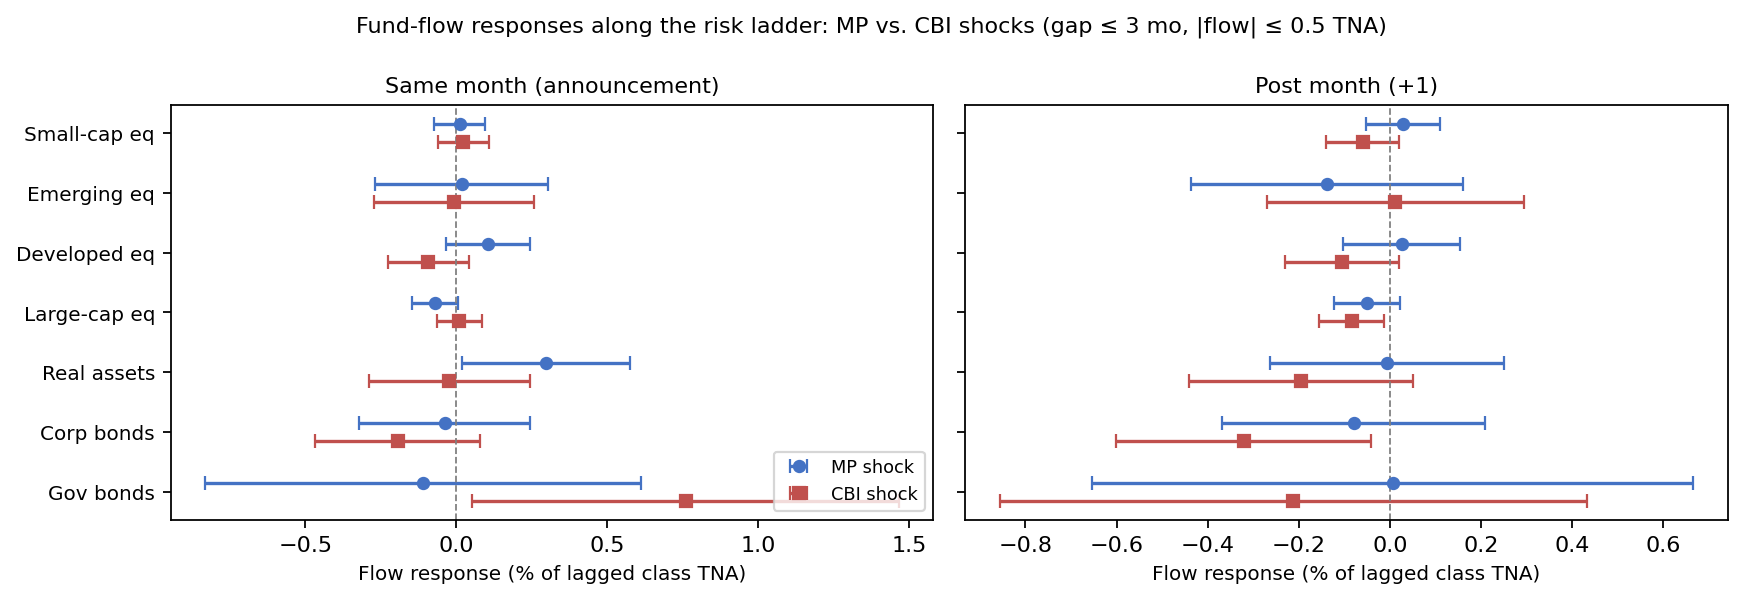
\includegraphics[width=0.94\textwidth]{figures/risk_ladder_v8.png}
  \vspace{0.2em}
  \begin{itemize}
    \item Same month: gov bonds $+0.76$ on CBI ($p=0.037$), $\approx 0$ on MP; Wald $p=0.098$
    \item Post month: \textbf{corporate bonds $-0.32$ ($p=0.026$)}, large-cap equity $-0.08$ ($p=0.022$) on CBI
    \item Diff window: gov bonds $-0.99$ ($p=0.014$) --- the safe-asset inflow is \emph{temporary}; de-risking follows
  \end{itemize}
  {\scriptsize\textcolor{gray}{Caption: flow responses (\% of lagged class TNA) with 95\% CIs, OLS, classical SEs; gap $\leq$ 3 months, $|$flow$| \leq 0.5$ TNA; controls included.}}
\end{frame}

% ---- 10. Hypothesis B + Result ----
\begin{frame}{10. Hypothesis B: flows shift along the risk ladder}
  \begin{aalertblock}{$H_B$ (revised): information revelations trigger \emph{de-risking}}
    \begin{equation}
      \mathrm{Risk}_{c}\times \mathrm{CBI}_t: \quad \beta_4 < 0
    \end{equation}
    Pooled panel over the 7-class ladder (rank 1 = gov bonds \ldots 7 = small-cap equity).
  \end{aalertblock}
  \begin{itemize}
    \item Found: $\beta_4 = -0.066$ ($p = 0.036$); gap-free variant $-0.114$ ($p=0.002$) --- same sign, $\sim$40\% larger
    \item Risk$\times$MP is flat ($p=0.88$): policy actions do not reorder the ladder
    \item \textbf{This is a direction reversal} of the original proposal (risk-seeking) --- reported as found; intraday flows would discriminate ``prediction wrong'' vs.\ ``monthly masks faster reallocation''
  \end{itemize}
  {\scriptsize\textcolor{gray}{Caption: Hypothesis B with the revised sign, the evidence, and the honest caveat.}}
\end{frame}

% ---- 11. Hypothesis C ----
\begin{frame}{11. Hypothesis C: wording matters for prices only under forward guidance}
  \begin{agreenblock}{A real forward-guidance sentence (Aug 9, 2011 statement)}
    ``\ldots are likely to warrant exceptionally low levels for the federal funds rate \textbf{at least through
    mid-2013}.''
  \end{agreenblock}
  \begin{columns}[T]
    \column{0.52\textwidth}
    \begin{itemize}
      \item Regression: same-day CRSP VW $\sim$ shocks $\times$ FG regime
      \item \textbf{Found:} tone $\beta = -1.01$ per 100 net words ($p=0.005$), model $R^2 = 32.8\%$ ($N=56$) in
            FG; $p=0.35$ outside. When rates are stuck, words are the tool.
      \item Caveat: tone itself is not significantly linked to either shock ($p=0.36$) --- it works as language,
            not as a shock proxy
    \end{itemize}
    \column{0.44\textwidth}
    \begin{ablock}{What this changes}
      This result was buried mid-deck; it is now the second contribution. It survives every correction made in
      the October audit.
    \end{ablock}
  \end{columns}
  {\scriptsize\textcolor{gray}{Caption: Hypothesis C (current H3) with one genuine statement quote and the surviving result.}}
\end{frame}

% ---- 12. Timing (optional) ----
\begin{frame}{12. Timing: who trades first? (optional)}
  \begin{itemize}
    \item Prices move on the announcement day; flows adjust over the following month
    \item Consistent with fast institutions repricing and slower retail money following
    \item Same-month gov-bond inflow reverses by $+1$ month (Diff $-0.99$, $p=0.014$): the safe-asset bid is
          transient, the de-risking is not
    \item Next step: intraday/weekly flow data to order the two margins directly
  \end{itemize}
  {\scriptsize\textcolor{gray}{Caption: the timing page --- prices first, portfolios later, and the one-month reversal.}}
\end{frame}

% ---- 13. Fixing and plan ----
\begin{frame}{13. What I'm fixing, and the plan}
  \footnotesize
  \begin{tabularx}{\textwidth}{l X l}
    \toprule
    \textbf{Item} & \textbf{Action} & \textbf{Status} \\
    \midrule
    Sample & Statements-driven, 161 meetings, 2006--2026 & \textbf{done} \\
    Returns & Same-day CRSP, percent units & \textbf{done} \\
    Statement texts & Body-only; 2 documents re-fetched & \textbf{done} \\
    Flows & WRDS re-run, point-in-time classes, gap rule & \textbf{done} \\
    Outlier rule & $|$flow$| \leq 0.5\times$TNA (replaces no-op filter) & \textbf{done} \\
    Pseudo B--S step & Removed; shocks in native form & \textbf{done} \\
    LLM measure & Rebuild to read statement text (current score does not) & in progress \\
    Dictionary & Scale LM/CB lists to stated sizes & in progress \\
    Robustness & Bauer--Swanson (real), intraday shocks & planned \\
    \bottomrule
  \end{tabularx}
  {\scriptsize\textcolor{gray}{Caption: the audit-fix table; everything above the line is already in these slides.}}
\end{frame}

% ---- 14. Contributions recap ----
\begin{frame}{14. Contributions, again, in three lines}
  \begin{enumerate}
    \item First evidence that \textbf{rate news vs.\ economy news move mutual-fund money differently} ---
          safe-asset inflows on information shocks, de-risking along the ladder
    \item \textbf{Tone matters only under forward guidance} --- statement language prices only when rates cannot
    \item A \textbf{corrected, reproducible pipeline} --- and an interactive research platform --- behind every number shown today
  \end{enumerate}
  {\scriptsize\textcolor{gray}{Caption: the recap --- what a reader should take away, matching slide 4.}}
\end{frame}

% ---- 15. Thank you ----
\begin{frame}{15. Thank you}
  \begin{ablock}{Backup available on request}
    Null results (tone--surprise regressions, incremental $R^2$) $\cdot$ robustness across gap rules and caps
    $\cdot$ variable construction tables $\cdot$ data-corrections appendix
  \end{ablock}
  \centering
  \vspace{0.6em}
  \textbf{What Moves Money: Rate News vs.\ Economy News}\\
  \small 161 FOMC meetings, 2006--2026 \quad$\cdot$\quad CRSP mutual funds \quad$\cdot$\quad all numbers reproducible
\end{frame}

% ---- Backup ----
\appendix

\begin{frame}{Backup B1: null results, stated plainly}
  \footnotesize
  \begin{tabularx}{\textwidth}{l X}
    \toprule
    \textbf{Hypothesis} & \textbf{Result on corrected data} \\
    \midrule
    Tone $\sim$ Target/Path (current $H_1$) & $\beta_T = +0.08$ ($p=0.36$), $\beta_P = +0.01$ ($p=0.92$); Wald(Target=Path) $p=0.59$. Tone is descriptive. \\
    Incremental $R^2$ (current $H_2$) & $+0.16$ pp ($p=0.64$), 2006--2022; $+0.82$ pp ($p=0.26$) full sample. Earlier marginal significance came from next-day alignment. \\
    Implication & These are reported as nulls; the paper leads with flows (H4/H5) and FG (H3), where the data are strong. \\
    \bottomrule
  \end{tabularx}
  {\scriptsize\textcolor{gray}{Caption: the nulls, so the meeting never discovers them unannounced.}}
\end{frame}

\begin{frame}{Backup B2: robustness across flow specifications}
  \footnotesize
  \begin{tabularx}{\textwidth}{l l l l}
    \toprule
    & \textbf{Gap-free, cap 1.0} & \textbf{Gap $\leq$ 3 mo, cap 0.5 (main)} & \textbf{Reading} \\
    \midrule
    Gov bonds, CBI (same) & $+1.13$ ($p=0.010$) & $+0.76$ ($p=0.037$) & same sign \\
    Corp bonds, CBI (post) & --- & $-0.32$ ($p=0.026$) & de-risking \\
    Risk$\times$CBI & $-0.114$ ($p=0.002$) & $-0.066$ ($p=0.036$) & same sign \\
    MP$\times$ZLB & $-0.96$ ($p=0.12$) & $-1.51$ ($p=0.005$) & sharper under the cap \\
    \bottomrule
  \end{tabularx}
  {\scriptsize\textcolor{gray}{Caption: signs and significance are preserved; magnitudes shrink $\sim$40\% under the measurement-error fix.}}
\end{frame}

\begin{frame}{Backup B3: variable construction}
  \footnotesize
  \begin{tabularx}{\textwidth}{l X}
    \toprule
    \textbf{Variable} & \textbf{Construction} \\
    \midrule
    Target / Path shock & FF / ED futures in a narrow window around 2:00pm FOMC releases (GSS 2005) \\
    MP / CBI split & Sign restriction on same-day equity return (JK 2020 logic), 91 MP / 60 CBI meetings \\
    Tone & LM hawkish minus dovish, per 100 words, body-only statement text \\
    Flow$_{c,t}$ & $\sum_f \big[\mathrm{TNA}_{f,t} - \mathrm{TNA}_{f,t-1}(1+r_{f,t})\big] \big/ \sum_f \mathrm{TNA}_{f,t-1}$ within class $c$ \\
    FG regime & Dec 16, 2008 -- Dec 15, 2015 (calendar-based; robust to date-based definitions) \\
    ZLB regime & Mar 15, 2020 -- Jan 26, 2022 \\
    \bottomrule
  \end{tabularx}
  {\scriptsize\textcolor{gray}{Caption: every variable, one line each.}}
\end{frame}

\end{document}
